\documentclass[addpoints, answers]{exam}

\usepackage{amssymb, amsmath, amsfonts}
\usepackage{geometry}
\usepackage{graphicx}
\usepackage{tikz}
\usetikzlibrary{calc}
\usepackage{pgfplots}
\usepackage{multirow,array} % for payoff matrix formatting

\definecolor{crimson}{RGB}{ 170, 4, 36 }
\definecolor{darkblue}{RGB}{ 4, 47, 170 }
\definecolor{brown}{RGB}{ 111, 71, 2 }
\definecolor{periwinkle}{RGB}{ 90, 177, 204 }
\definecolor{ducksgreen}{HTML}{007030}
\definecolor{darkgray}{RGB}{169, 169, 169}
\definecolor{dimgray}{RGB}{105, 105, 105}

\geometry{left=1.0in,right=1.0in,top=1.0in,bottom=1.0in}
\pagestyle{headandfoot}
\lhead{EC327 Game Theory}
\chead{Practice Midterm}
\rhead{Winter 2024}
\runningheadrule

\newcounter{BoSparts}
\title{
    \textbf{Econ 327: Game Theory} \\ 
    Practice Exam
    }
\author{University of Oregon}
\date{\today}

% exam-type question formatting
\renewcommand{\thequestion}{\textbf{Question \arabic{question}}}
\bracketedpoints

\begin{document}

\maketitle

\begin{center}
  \Large{\textbf{Version 1}}
\end{center}

\begin{center}
  \gradetable[h][questions]
\end{center}

% \vspace{0.5in}

% \begin{center}
%   \textbf{For homework assignments:}
% \end{center}
% 
% \begin{itemize}
% 
% %  \item DO NOT write your name:
% %  this assignment will be graded anonymously. 
% %  If you want to, you can include your student ID instead.
% 
%   \item Complete \textit{all} questions and parts.
%   I will select one question at random to be graded
%   according to the rubric on Canvas.
% 
%   \item You may choose to work with others,
%   but everyone must submit to Canvas individually.
%   Please include the names of everyone who you worked with 
%   below your own name.
%  
% \end{itemize}

\begin{center}
  \textbf{For Exams:}
\end{center}

\begin{itemize}
  
  \item Complete \textit{all} questions and parts. 
  All questions will be graded.

  \item Carefully explain all your answers on short and long answer questions.

  An incorrect answer with clear explanation will earn partial credit,
  an incorrect answer with no work will get zero points.

  \item 
  If you do not understand what a question is asking for, 
  ask for clarification. 

\end{itemize}

\underline{Allowed Materials:}

\begin{itemize}
 
  \item A single 5" by 3" note card

  \item A non-programmable calculator

  \item Pencils, color pens, eraser, ruler/straight-edge etc.
\end{itemize}

\vspace{1.0in}

\makebox[.6\textwidth]{Name\enspace\hrulefill}

\vspace{0.5in}

\begin{center}
  \fbox{\fbox{\parbox{5.5in}{\centering
    Answer the questions in the spaces provided on the
    question sheets. If you run out of room for an answer,
    continue on the back of the page or another sheet of paper.}}}
\end{center}

\newpage

\begin{questions}

%------------------------------------------------------------------%

\question[20] 

\section*{Multiple Choice}
\noindent\fbox{
  \parbox{\linewidth}{
  See the Quizizz from Tuesday for more practice.

  They will look like the multiple choice questions from homework,
  but there will be 10 total instead of 5.}
}


%------------------------------------------------------------------%
\section*{Long Answer}

%------------------------------------------------------------------

\question 

Giustina and Ne\v{z}a can each either go to dinner at 
  \textit{Lion \& Owl} or \textit{Spice N Steam}.
They both would prefer to go to a restaurant together than to go alone.
Giustina prefers \textit{Lion \& Owl} to \textit{Spice N Steam}, 
  but Ne\v{z}a prefers \textit{Spice N Steam} to \textit{Lion \& Owl}.
Giustina is the more decisive of the two, 
so she chooses a restaurant first
and then Ne\v{z} decides which restaurant she will go to 
after seeing where Giustina is going.

\begin{parts}

  \part[10] Draw an extensive form game to go with this story 
  and solve for all subgame perfect Nash equilibria. 

  \vspace{7cm}

  \part[10] 
  Now represent this game in strategic form
  and solve for all pure strategy Nash Equilibria.
  Can you find any Nash equilibria which are not subgame perfect?

  \setcounter{BoSparts}{\value{partno}}
  
\end{parts}

\newpage

Now suppose that if Giustina and Ne\v{z}a show up to \textit{Lion \& Owl} together,
there is a chance that they will have to wait up to an hour to get a table.
If they have to wait, Giustina would be equally happy going to \textit{Spice N Steam} 
together where they wouldn't have to wait. 
Ne\v{z}a would be equally waiting to go to \textit{Lion \& Owl} with Giustina
or \textit{Spice N Steam}
  
\begin{parts}\setcounter{partno}{\value{BoSparts}}
  
  \part[10] Draw a new extensive form game to match the updated story.
  Make sure to define any variables you include.

  \vspace{7cm}

  \part[10] Find all subgame perfect Nash equilibrium which results in both
  Giustina and Ne\v{z}a going to \textit{Spice N Steam}.

  Your answer should be a function of the probability of waiting in line at \textit{Lion \& Owl}.
\end{parts}

\newpage
%------------------------------------------------------------------

\question%[20]

Consider the strategic form game below:

\begin{table}[!h]
  \begin{center}
    \begin{tabular}{*{6}{c|}}
      \multicolumn{2}{c}{} & \multicolumn{4}{c}{$P_2$} \\ \cline{3-6}
      \multicolumn{1}{c}{} &  & $A$ & $B$ & $C$ & $D$ \\ \cline{2-6} 
      \multirow{4}*{$P_1$}
      & $W$ & 15, -7 &  8,  2 & 18, -7 & 11,  5 \\ \cline{2-6}
      & $X$ & -3, 18 &  6, -7 &  8, -7 & 17, 18 \\ \cline{2-6} 
      & $Y$ &  9, 19 & 20, -4 & 13,  6 & 10, 16 \\ \cline{2-6} 
      & $Z$ & -9, 20 & 14, 16 & 15, -5 & -3,  4 \\ \cline{2-6} 
  \end{tabular}
  \end{center}
\end{table}

\begin{parts}
 
  \part[8] 
  Use Iterated Deletion of Strictly Dominated Strategies
  and write out a simplified game table with any remaining cells.

  \vspace{50mm}

  \part[10]
  Find all Nash equilibria in \textit{pure strategies}.
  Explain why you know they are Nash equilibria.

  \vspace{50mm}
  
  \part[6] 
  Define mixed strategies for each player
  using any pure strategies left after IDSDS.
  Make sure to define all variables you introduce.

  \newpage 

  \part[8]
  Graph each player's expected utilities as functions of the 
  other players' mixed strategy you defined in part (c).

  \vspace{100mm}

  \part[8]
  Solve for all Mixed Strategy Nash equilibria in this game.
  A complete answer will include all calculations used 
  and a graph of best response functions.

  % blank page for work

\end{parts}

\newpage{\cleardoublepage}

\ 

\newpage

%------------------------------------------------------------------

\section*{Short Answer}

\noindent\fbox{
  \parbox{\linewidth}{These questions were cut for time on the actual midterm exam,
  but they are still good practice.

  Just don't count how much time you spend on them 
  when you're gauging how long the real exam will take you.}
}

\begin{parts}
\part
Consider the strategic form game below:

\begin{table}[h!]
  \begin{center}
  \begin{tabular}{*{5}{c|}}
    \multicolumn{2}{c}{} & \multicolumn{3}{c}{Aslanbek} \\\cline{3-5}
    \multicolumn{1}{c}{} & & $Low$ & $Moderate$ & $High$ \\\cline{2-5}
    \multirow{3}*{Hagano}  & $Low$ & 0,0 & 3,2 & 7,3 \\\cline{2-5}
                         & $Moderate$ & 2,3 & 5,5 & 6,4 \\\cline{2-5}
                         & $High$ & 3,7 & 4,6 & 4,5 \\ \cline{2-5}
  \end{tabular}
  \end{center}
\end{table}

Find all pure Nash strategy profiles.

\vspace{40mm}

%------------------------------------------------------------------

\part
Akua, Barta, and Gilberta are playing a version of hide and seek.
There are only two good hiding spots;
up a tree, or behind a rock.
Akua gets to hide first.
Barta also hides, but she gets to see which spot Akua is hiding
before she picks.
Once Akua and Barta are hidden,
Gilberta has to choose one and only one place to look.
If there are two people hiding in the same spot, 
they crowd each other and Gilberta can see them.
If there is only one person in a spot, Gilberta can't see 
who's hiding there.

Create an extensive form game tree
and clearly specify Gilberta's information set.

% \vspace{40mm}
\newpage

%------------------------------------------------------------------

\part
Suppose that two fishing boats are selling to the same market.
Let $V$ be the tons of fish caught by Vlatislav's boat,
and $J$ be the tons of fish caught by Jeren's boat.
People in this town only want to buy so many fish,
so the price $P$ of fish is given by the inverse demand function:
  $$P = 60 - (R+S)$$

Assuming both boat owners only care about profit, 
we get that Vlatislav's best response function is
  $$ V = 15 - \frac{J}{2} $$

and that Jeren's best response function is
$$ J = 12 - \frac{V}{2}$$ 

Graph both players' best response functions 
and find all Nash Equilibria.
Label your graph appropriately.

\vspace{10mm}

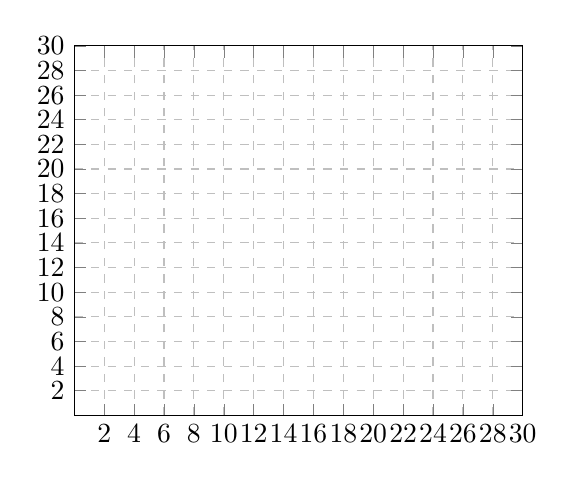
\begin{tikzpicture}

  \begin{axis}[
    width=0.6\textwidth,
    grid,
    % xlabel={Fish caught by Vlatislav ($V$)},
    % ylabel={Fish caught by Jeren ($J$)},
    xmin=0, xmax=30,
    ymin=0, ymax=30,
    xtick={2,4,...,30},
    ytick={2,4,...,30},
    grid style=dashed,
    ]

    \addplot[draw=none] coordinates {(1,1)};

  \end{axis}
\end{tikzpicture}
\newpage

\end{parts}

%------------------------------------------------------------------



\end{questions}

\end{document}
